\documentclass[10pt,a4paper, bibliography=totoc]{scrartcl}
\usepackage[utf8]{inputenc}
%\usepackage[nenglish]{babel}
\usepackage{amsmath}
\usepackage{amsfonts}
\usepackage{amssymb}
\usepackage{marvosym}
%\usepackage{gensymb}
\usepackage{graphicx}
\usepackage{hyperref}
\usepackage{url}
\usepackage{float}
\usepackage{siunitx}
\DeclareSIUnit{\Greatmol}{M}
\usepackage{bookmark}
\usepackage{booktabs}
%\sisetup{locale = DE}
\usepackage{subcaption}
\usepackage{listings}
\usepackage{xcolor}

\definecolor{codegreen}{rgb}{0,0.6,0}
\definecolor{codegray}{rgb}{0.5,0.5,0.5}
\definecolor{codepurple}{rgb}{0.58,0,0.82}
\definecolor{backcolour}{rgb}{235, 235, 235}

\lstdefinestyle{mystyle}{
    backgroundcolor=\color{backcolour},   
    commentstyle=\color{codegreen},
    keywordstyle=\color{magenta},
    numberstyle=\tiny\color{codegray},
    stringstyle=\color{codepurple},
    basicstyle=\ttfamily\footnotesize,
    breakatwhitespace=false,         
    breaklines=true,                 
    captionpos=b,                    
    keepspaces=true,                 
    numbers=left,                    
    numbersep=5pt,                  
    showspaces=false,                
    showstringspaces=false,
    showtabs=false,                  
    tabsize=2
}
\lstset{style=mystyle}
\lstset{literate=%
  {Ö}{{\"O}}1
  {Ä}{{\"A}}1
  {Ü}{{\"U}}1
  {ß}{{\ss}}1
  {ü}{{\"u}}1
  {ä}{{\"a}}1
  {ö}{{\"o}}1
}
\usepackage[title,titletoc]{appendix}
\renewcommand{\appendixtocname}{Anhang}
\renewcommand{\appendixpagename}{Anhang}

\usepackage{caption}
\captionsetup{font=small}

%\renewcommand{\UrlFont}{\small\tt}
\usepackage[a4paper,lmargin={2.5cm},rmargin={2.5cm},tmargin={2.5cm},bmargin = {2.5cm}]{geometry}

\linespread{1.1}

\begin{document}

\pagenumbering{Roman}

\title{Ultrafast X-Ray Experiments}
\subtitle{Virtual Experiments at the X-Ray Laser European XFEL\\ Versuch EXP21}
\author{Léonie Lanz \\ Nico Kalogerakis}
\maketitle
\newpage

\tableofcontents
\vfill
\newpage

\pagenumbering{arabic}

\section{Einleitung}


\section{Theoretical Background}

\subsection{Synchrotronradiation}
When accelerating electrons or other charged particles to relativistic speeds along a curved trajectory they emit so-called synchrotron radiation. It gains is name from the ring accelerators, the sychrotrons, where it was first observed. A typical synchrotron facility consists of a linear accelarator leading into a booster ring in which the electrons are brought up to relativistic speeds \cite{1}\cite{3}. The electrons are then fed into a storage ring in which they continue to circulate at relativistic speeds. From the storage ring the beam-lines lead tangentially away in which the synchrotron radiation is utilized in experimental hutches \cite{1}\cite{3}. 
Synchrotron radiation is bright X-radiation with a wide tunability in energy, which is useful for examining structures and dynamics of materials, as x-ray photons have energies in the order of several kiloelectronvolts (keV) \cite{3}. This means their wavelengths are in the order of magnitude of Angstroms and comparable to the spacing of atoms in solid materials. This is useful, as it means that atoms in a crystalline array can diffract x-ray beams and the interference patterns can be measured \cite{1}.\\\\
There are four generations of synchrotrons with the main difference being the brilliance achieved \cite{1}. The first was the bending magnet in the synchrotron as it was used for high energy collider physics with no additional modifications. The second generation introduced the wiggler, a configuration of dipolmagnets with alternating polarity to achieve synchrotron radiation a linear path. The third generation synchrotron radiation facilities were designed for low emittance of the beams with more effective linear magnet configurations, the undulators \cite{3}. A low emittance means a smaller angular divergence of the beam and a higher brilliance \cite{3}.

\subsubsection{Free Electron Laser (FEL)}
Free-electron lasers are coherent tradiation sources that are capable of even higher brilliance than third generation synchrotron facilities \cite{2}. They are in theory able to operate at any arbitrary wavelength or spectrum of wavelength with the limit being the energy and quality of the accelerated electron beam \cite{2}. \\
They use a process called self-amplified stimulated emission (SASE). SASE free-electron lasers typically use monochromatic electron beams with a long, high-quality undulator around the order of magnitude of a few hundert metres. The light waves emitted by the electron bunches will line up in place and amplify themselves through superposition. As the electrons oscillate down the undulator they are also interacting with the magnetic components of the light they themselves are generating. The transverse component of the electrons oscillation and the magnetic field component pf the emitted light create a Lorentz force which acts upon the electrons and moves them along axial directions. This leads to the electrons creating microbunches inside their conventional bunches \cite{1}.\\\\
The duration of a single X-ray pulse can also be reduced to even less than a few femtoseconds. This allows for an investigation of molecular processes and photochemical reactions through a form of sequential snapshots with a characteristic time of under a picosecond \cite{1}.

\subsection{Pump-probe-principle}
The principle of pump-probe-spectroscopy is sending two lasers at the same object with a certain time delay so that the first laser, an optical laser, can excite the system in some way and the second laser, an X-ray pulse can measure the response (see \autoref{fig:pump probe}). In a FEL such as the European XFEL this can be done with ultrafast X-ray pulses on a timescale of a few femtoseconds ($\qty{e-15}{s}$). Variating the time delay allows for a series of sequential snapshots of the process observed and variating the wavelength of the excitation laser allows for an investigation of different processces \cite{0}.\\
The selection of the different discrete time delays is important. For negative time delays ($\Delta t<0$) the probe pulse arrives before the pump pulse and thus measures just the ground state and for a delay of $\Delta t=0$ both pulses overlap exactly. Whereas for positive delays ($\Delta t>0$) the probe pulse measures the developing dynamics.

\begin{figure}[h]
     \centering
     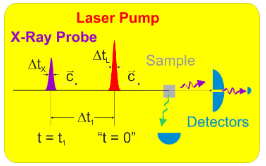
\includegraphics[scale=0.8]{img/pump probe 1.png}
     \caption{A schematic of a pump-probe-experiment \cite{0}.}
     \label{fig:pump probe}
\end{figure}

\subsubsection{The pump-pulse}
The pump pulse acts as a kick-off signal for the process. It excites the molecule at a well-defined time ($t=0$) from it's thermal ground state into a higher energetic state.\\
In this experiment specifically the pump pulse is an ultra-short optical laser-pulse with a wavelength in the VIS/UV range which excites the iron-compound $[\text{Fe}(\text{bipy})_3]^{2+}$ from it's singlet low-spin-state ($^1A_1$) into the excited state $^1\text{MLCT}$ (metal-to-ligand charge transfer). This starts the photophysical reaction.

\subsubsection{The probe-pulse}
The probe pulse is a second pulse that hits the probe with a known time delay to 'photograph' the current state. In this experiment an ultra-short X-ray pulse from the European XFEL is used. It ionises the 1s core electron of the central iron atom. The resulting X-ray emission ($K\beta$-XES) is measured which is sensitive to spin- and structure changes of the iron.

\subsubsection{Transient difference spectrum}
Most of the time during the experiment, only a fraction of the molecules in the probe are in an excited state. This means the pure excited spectrum is hard to see directly. To get a useful reading of the data the transient signal in the difference spectrum is used:
\begin{align}
\text{transient signal}=I_{\text{laser on}}(\Delta t)-I_{\text{laser off}}
\end{align}
The transient signal shows the physical changes the best: Negative parts of the signal mean a depopulation - places in the spectrum where the intensität lessened as the ground state was emptied because of the laser, positive parts are new spectral features such as the growing of a spin-sensitive satellite peak which indicates the existance of intermediate states.\\
When plotting the intensity of these notable energies against the time delays, you get so-called kinetic traces from which the lifespans of the intermediate states is able to be determined.

\subsection{The investigated molecule}
We investigated a molecule formed of an Iron center ($Fe^{2+}$), a transition metal ion, and 3 attached ligands (bipyridine). This forms a chemical complex compound. 
The central atom acts as an electron acceptor, while the ligand acts as the electron donor.

\begin{figure}[h]
     \centering
     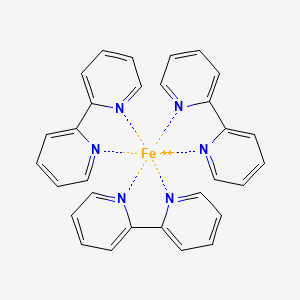
\includegraphics[scale=0.5]{img/tris(2,2'-bipyridine)iron(II).png}
     \caption{Schematic view of $[\text{Fe}(\text{bipy})_3]^{2+}$}
     \label{fig:schem bipy}
\end{figure}

This bonding can take place because of the $d^6$ electron configuartion of $Fe^{2+}$ and the nitrogene atoms in the pyridine rings. In our case we have two bridged pyridine rings that form the uncharged bidentate ligand bipyridine (abbreviated bipy). Both nitrogen atoms in each of the 3 ligands bind to the central $Fe^{2+}$ atom.

\subsubsection{Electronic Structure of \([Fe(bipy)_{3}]^{2+}\)}
Because of the electrostatic interaction between the ligands and the d electrons of the $Fe^{2+}$, the 5 d orbitals, that normally would be energetically equivalent, with a maximised spin multiplicity, are now energetically raised or lowered due to the nature of interaction with the ligand field. 
the energy of d orbitals pointing to the ligands ($e_g$) is raised, while the energy of those pointing between the ligands is lowered ($t_{2g}$). 
The difference of energy $\Delta_{oct}$ is called the strength of the crystal field.

\subsubsection{High spin and low spin states}
Following Hund's rule the lower-energy orbitals ($t_{2g}$) are filled first (one by one with electrons of the same spin).
In the low-spin state our $d^6$ metal ion has no unpaired electrons (total Spin $S=0$). That represents the singlet state $^1A_1$. 
In the high spin state it has the maximum of unpaired electrons ($S=2$). We habe a quinted state $^5T_2$.
The energy difference $\Delta_{oct}$ is smaller for HS configs, because the $e_g$ level is filled and those electrons can push the ligand atoms further away that in LS configs. 
Excitation to the HS state occurs in this experimental setup through photoexcitation to higher lying MLCT bands followed by relaxation.

\section{Experimental Setup}
The entrire experiment is conducted in VLab, a software modeled after a hutch in the experimental hall of the European XFEL in Schenefeld. The European XFEL is \qty{3.4}{km} long and runs from the DESY research center to the European XFEL campus. A \qty{1.9}{km} long superconducting linear accelerator feeds electrons with energies up to \qty{17.5}{GeV} into a branched tunnel system with two \qty{212}{m} long undulators that generate hard X-radiation in the range of \qty{5}{keV} to \qty{25}{keV} and one \qty{125}{m} long undulator that generates soft X-radiation in the range of \qty{0.25}{keV} to \qty{3}{keV}.\\\\
VLab recreates the Femtoseconf X-ray Experiment research platform. 

Datenstruktur (beam imaging and xray eye): 420x420 pixel, bei biu screen dim von 10mm x10mm, bei xray eye screen 2mm x 2mm

For further elaboration see \autoref{Anh: VLab}.
\subsection{Undulator and Beamline}
\subsection{Monochromator and Focusing Optics}
monochromator 
focusing optics: mirrors,  power slits, solid attenuators, refractive Lenses, X-ray eye
\subsection{Spectrum Analyser}
diffraction gratings
\subsection{Time-arrival Detector}
\subsection{Sample Environment}
\subsection{Laser System}
\subsection{Von Hamos Spectrometer}

Quelle Versuchsmappe:\cite{0}


\section{Experimental Procedure}
\subsection{Preparation of the Experiment}
\subsubsection{Alignment and Characterization of the X-ray Beam}
Before doing anything on a beam line it's important to characterize it.\\
As the absorption edge for the Fe K$\beta_{1,3}$ line of 7065 eV, the energy of the xray beam is set to 7400 eV, to avoid the ripples near the reaction (as illustrated by the X-ray absorption spectrum of $[\text{Fe}(\text{terpy})_2]^{2+}$ \autoref{fig:xas terpy}) but without too strong of a loss in intensity.\\
\begin{figure}[h]
     \centering
     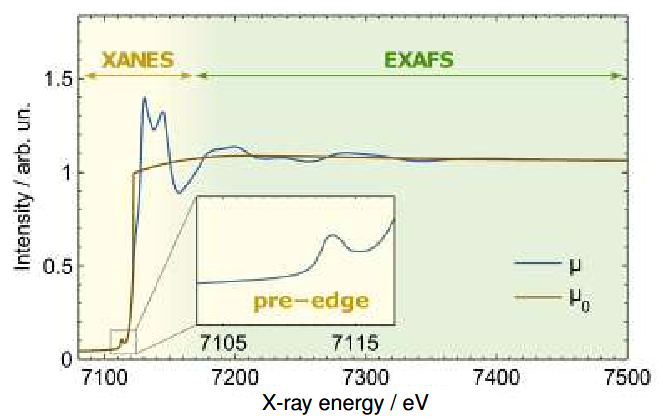
\includegraphics[scale=0.5]{img/xas terpy.png}
     \caption{X-Ray absorption spectrum of $[\text{Fe}(\text{terpy})_2]^{2+}$ (terpy: terpyridin) at the Fe K edge displaying the XANES and EXAFS regions including the background absorption contributions $\mu_0$. The inset zooms into the weak pre edge features \cite{0}.}
     \label{fig:xas terpy}
\end{figure}

To measure the initial X-ray beam the power slits are fully opened and the following attenuator foils are used to bring the beam to an intensity just below saturatuion of the beam imaging unit 2 (BIU2): 
\begin{table}[H]
    \centering
    \caption{Attenuator foils used}
    \label{tab:atten initial}
    \begin{tabular}{|S|S|}
        \toprule
        {Rod} & {Attenuator foil} \\
        \midrule
        1 & {C }0.1 \\
        2 & {--} \\
        3 & {Si }0.1 \\
        4 & {B4C }0.8 \\
        \bottomrule
    \end{tabular}
\end{table}

The size and position of the x-ray is now measured using BIU2. %do we want the pictures here?
Then the four-bounce crystal-monochromator is turned on and then off again to record the reduction of the spectral bandwidth. Then the dispersive single-shot spectrum analyser is used to record the spectrum of the pink X-ray beam with a bragg angle of 24°. \\
For the following experiment the pink X-ray beam is used even though the monochromatic has a higher resolution, as the intensity of the beam suffers about three orders of magnitude under the monochromator.\\\\

The last step of diagnosing the beam line is using the refractive beryllium x-ray lenses to focus the beam at the imaging unit x-ray eye. It's important to appropiately adjust the attentuator foils as to not burn the imaging unit with a focussed beam. 

\begin{table}[H]
    \centering
    \caption{A list of the beryllium lenses available in VLab together with the arms they were mounted on (arm 10 the most downstream), the Number of lenses in each cassette $N$ and the central curvature of the lenses $R$ \cite{0}.}
    \label{tab:lenses}
    \begin{tabular}{|c| c c c c c c c c c c|}
        \toprule
        {\textbf{Arm}} & 10 & 9 & 8 & 7 & 6 & 5 & 4 & 3 & 2 & 1 \\
        \midrule
        {\textbf{N}} & 10 & 10 & 8 & 7 & 5 & 9 & 4 & 10 & 6 & 1 \\
        {\textbf{R/mm}} & 0.5 & 0.5 & 0.5 & 0.5 & 0.5 & 1.0 & 0.5 & 1.5 & 1.5 & 0.5\\
        \bottomrule
    \end{tabular}
\end{table}

With beryllium lenses 1, 2 and 5 (taken from \autoref{tab:lenses}) and appropiate attenuator foils inserted, a beam with the FWHM of ~13 um (siehe \autoref{fig:strahlbreite}) is achievd. The total focus length is calculated with $\delta \approx 7\cdot 10^{-6}$ \cite{0} and the properties of the lenses themself taken from \autoref{tab:lenses}:
\begin{align*}
	F=\frac{R}{2\delta N} &\Leftrightarrow \frac{1}{F_{ges}}=\frac{2\delta N_1}{R_1}+\frac{2\delta N_2}{R_2}+\frac{2\delta N_5}{R_5}\\
	&\Leftrightarrow F_{ges}=\frac{1}{2\delta(\frac{N_1}{R_1}+\frac{N_2}{R_2}+\frac{N_5}{R_5})} \approx \qty{4,76}{m}
\end{align*}

\begin{figure}[h]
     \centering
     %grafik muss gefixed werden :/
     
\includegraphics[scale=0.5]{img/FWHM_gaussian.png}
     \caption{The horizontal and vertical profile of the focussed X-ray beam plotted together with a gaussian fit and the corresponding FWHM of \qty{13.5}{\mu\m}.}
     \label{fig:strahlbreite}
\end{figure}

---Notes---

X-ray energy \(E_0=7400eV\) (has to be a good bit away from reaction edge of 7065 keV to be stable)

Alignment:
attenuators to not burn through out screens (here: 4: B4C 0.8, 3: C 0.4, 2: Si 0.05, C 0.1)
size and position of the beam plots (FWHM) (jitter neu!)
pink vs mono beam 2D/3D plots

optical resolution: ~25 um/px

Characterization:
spectrum of the pink vs mono beam plots
myb noch ex 7+8, aber idk

Focusing:
plots of the focused beam size and position (FWHM)

\subsubsection{Preparatory Estimates for the Experiment}
The transition metal complex $[\text{Fe}(\text{bipy})_3]^{2+}$ to be studied is obtained through dissolving the salt $[\text{Fe}(\text{bipy})_3]\text{Cl}_2$ in deionized water to the desired concentration. As the actual sample is a powder consisting of small microcrystals that contain incorporated water which remained in the crystal lattice after the crystallization process.\\
A minimum volume of \qty{50}{ml} is required to operate the liquid jet in the experiment. To ensure that the sample is completely refreshed between probe pulses, the jet needs to have a certain flow speed with an assumed repition rate of the X-ray pulse train of \qty{1.1}{MHz} and an assumed top hat beam profile of the X-ray laser with the dimension $\qty{10}{\micro\m}\times\qty{10}{\micro\m}$. The minimum required flowspeed is calculated as follows:
$$\Delta x_{\text{travel}} \ge w \quad \Rightarrow \quad v_{\text{min}} \cdot \Delta \tau \ge w \quad \Rightarrow \quad v_{\text{min}} \ge \frac{w}{\Delta \tau}\Rightarrow v_{\text{min}}=\qty{11}{\m\per\s}$$
With $w=\qty{10}{\micro\m}$ being the spatial width and $\Delta\tau=\frac{1}{f}=\frac{1}{\qty{1.1e6}{Hz}}\approx\qty{9.09e-7}{s}$ the characteristic time.\\\\
There are three laser wavelengths available for excitation: \qty{355}{nm}, \qty{400}{nm} and \qty{515}{nm}. To evaluate which fits the experiment best, the concentration $c$ of the solution for the three wavelengths for a desired optical density of $OD=1$ and a liquid jet thickness of $d=\qty{25}{\mu\m}$.
The optical density is defined as $OD=\epsilon\cdot c\cdot d$ with $\epsilon(\lambda)$ the wavelength dependent extinction coefficient of $[\text{Fe}(\text{bipy})_3]^{2+}$ in water. The extinction coefficients can be estimated to be $\epsilon(\qty{355}{nm})=\qty{12000}{\per\Greatmol\per\cm}, \epsilon(\qty{400}{nm})=\qty{4000}{\per\Greatmol\per\cm}, \epsilon(\qty{515}{nm})=\qty{8000}{\per\Greatmol\per\cm}$ as taken from \autoref{fig: ext coeff}.\\
\begin{figure}[h]
     \centering
     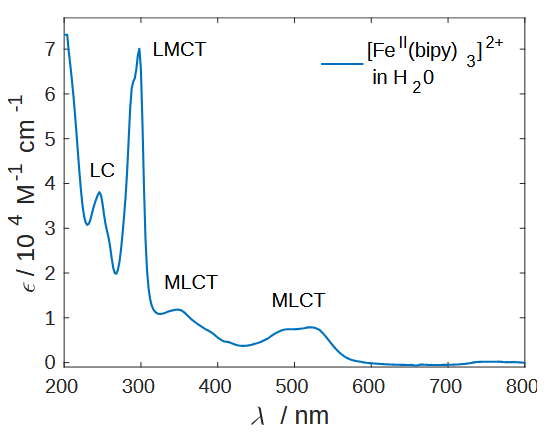
\includegraphics[scale=0.5]{img/abs spec aqu sol.png}
     \caption{UV/VIS absorption spectrum of an aqueous $[\text{Fe}(\text{bipy})_3]\text{Cl}_2$ solution. The
different CT transitions are indicated. The measured molar absorptivity $\epsilon$ values lie in the
expected range of $10^{-4}\text{\, l}\text{\,mol}^{-1}\text{\,cm}^{-1}$ to $10^{-5}\text{\, l}\text{\,mol}^{-1}\text{\,cm}^{-1}$ for dipole-allowed transitions\cite{0}}
     \label{fig: ext coeff}
\end{figure}
The following concentrations were calculated:
$$c_{355}=\qty{0.033}{mol\per\l}, c_{400}=\qty{0.100}{mol\per\l}, c_{515}=\qty{0.050}{mol\per\l}$$
There are different pulse energies available for each excitation wavelength: \qty{5}{\mu\J}(\qty{355}{nm}), \qty{15}{\mu\J}(\qty{400}{nm}) and \qty{50}{\mu\J}(\qty{515}{nm}). With that in mind the wavelangth of \qty{400}{nm} was chosen, as it has a higher pulse energy, even though it's not ideal when looking at the low absorption rate. The extinction coefficien of the \qty{515}{nm} is slightly better but with the low pulse energy it will be hard to see anything.\\\\

As we want to ensure that the X-ray beam always hits excited molecules we need to determine the diameter of the optical laser beam as well as the diameter of the X-ray beam correctly in relation to each other. 
%The optical laser beam profile is approximately Gaussian-shaped and has an original diameter of \qty{10}{mm} (FWHM). This collimated beam is focussed onto the liquid jetz by a lens with a focal length of $f=\qty{250}{mm}$. From the Rayleigh criterion $d_{Airy}=2.44\cdot \frac{\lambda\cdot f}{D}$ we calculate $d_{Airy}=\qty{24.4}{\mu\m}$ or rather $d_{FWHM}=?$ with our chosen wavelength of \qty{400}{nm}.
If the optical laser and the X-ray laser had the same diameter, the x-ray would also investigate molecules that were excited only weakly or even not at all, as the optical laser has an approximately Gaussian beam shape. Ideally, the X-ray is positioned exactly in the centre of the ca. 10 times bigger optical laser beam. Then it can investigate a maximal volume of excited molecules. This also compensates for the fact that the optical laser jitters in the focus layer of the X-ray due to not being focussed there itself.\\
These estimates have consequences for our needed flow speed of the liquid jet which has to be 10 times faster to adjust to the new diameter of the optical laser.\\\\
Ideally, the number of absorbed optical laser photons should be less than or approximately equal to the number of sample molecules in the laser-excited volume. This reduces the likelyhood that multiple photons hit the same molecule and excite it into states other than the one we want to observe while still optimizing the number of excited molecules. 
%hier muss noch der abschnitt 19 erläutert werden

There are two X-ray crystal spectrometers available to use: a von Hamos spectrometer and a Johann spectrometer. As the von Hamos spectrometer can record the entire spectrum at once while also being immune to intensity variation, in contrast to the Johann spectrometer which needs to scan each wavelength seperately and requires normalization to the sáccumulated incident intensity at each measurement point to measure the whole spectrum, it is better suited for this experiment.\\\\
In order to choose the correct crystal for the emission spectrometer the Bragg reflection angle needs to be considered. 
%hier fehlt noch der Prozess der Kristall-auswahl mit bragg und so

%Fun Facts: molar mass: \(M([Fe(bipy)_3]^{2+})\approx M([Fe(bipy)_3])=524,409 \frac{g}{mol}\), concentration of the sample: \(c=0,380\frac{mol}{L}\), total attenuation of X-rays: attenuation comparison plot, flow speed of the jet: \(v_{jet}=11\frac{m}{s}\)
%Laser: excitation wavelength: \(\lambda_{pump}=400nm\) (dazu alle fun facts mit MLCT Zuständen und so, und nicht overshooten lol), focussing,  diameter of the focus, Overfilling: beam sizes of the optical laser and the X-ray pulse relative to each other (plot beam diameter)
%Spectromter: Van Hamos Spectrometer vs Johann Spectrometer (plot of the two geometries), crystal selection: \(Si(531)\) vs \(Ge(531)\) (plot of the two crystal reflections)

\subsection{Performing the Experiment with Data Acquisition}
Using the Large Pixel Detector one can optimize the position of the liquid jet in the X-ray beam for maximal intensity of elastic scattering. The maximal intensity achieved with a pink beam was $3.8\cdot10^{15}$.\\
The X-ray emission spectrometer was adjusted by setting the Bragg angle range to ... and orienting the detector perpendicular to the incoming dispersive spectrum (see \autoref{fig:von hamos}).
\begin{figure}[h]
     \centering
     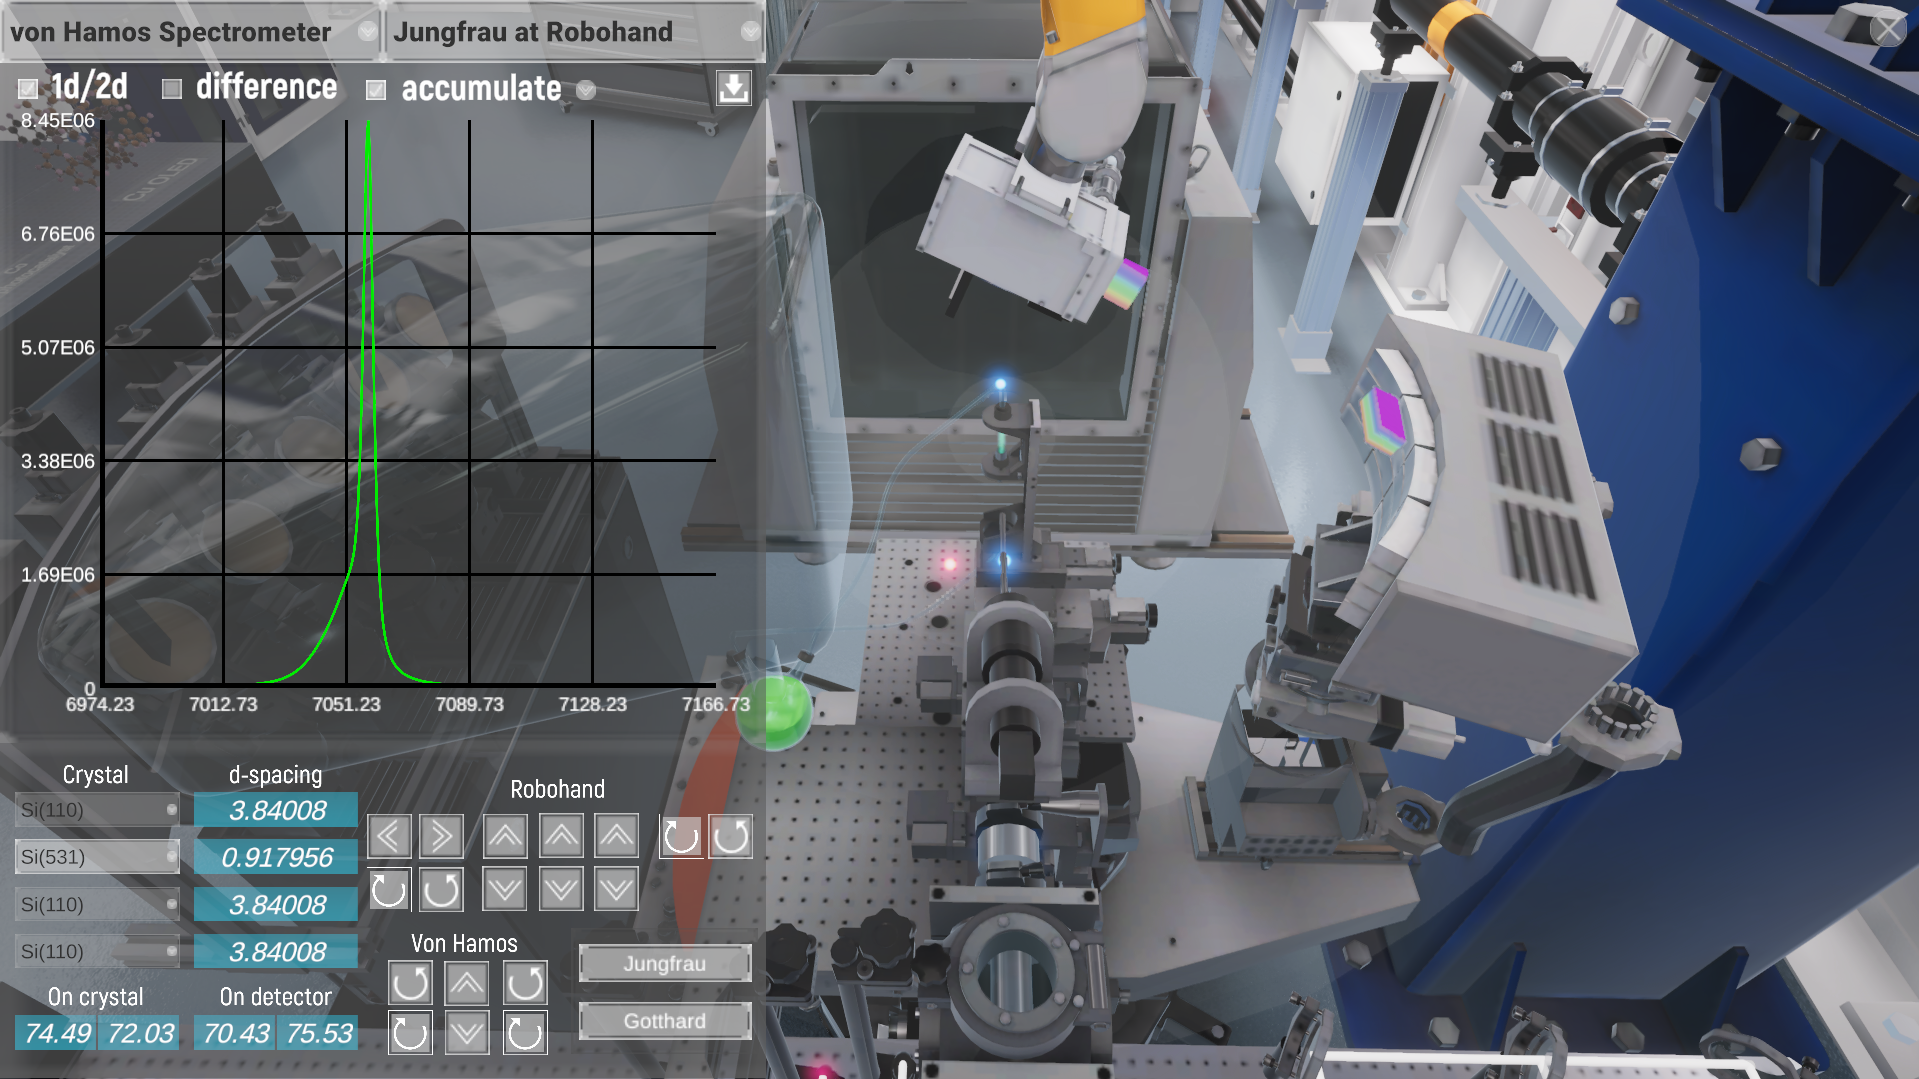
\includegraphics[scale=0.2]{img/100 ps Screenshot 2026-09-03 093257.png}
     \caption{The Von Hamos spectrometer in operating position. with the read-out of the Jungfrau detector as well as the settings for the position to the left.}
     \label{fig:von hamos}
\end{figure}

%couldnt find the kb1,3 spectrum :( but that still needs to be inserten here

The excitation laser was set to $\lambda=\qty{400}{nm}$ and $f=0.02$ with a beam diameter of $d=\qty{150}{\mu\m}$ in the sample plane. The spatial overlap between laser and X-ray beam was adjusted so that the X-ray laser always overlapped with the optical laser even with the jitter of the optical laser.

%pictures picture pictures

First the time delay of the laser was set to \qty{100}{ps}. This time delay means the laser pulse definitely strikes the sample before the X-ray pulse arrives. XES spectra with the laser on and off were recorded, as well as a difference spectrum.

For the main measurement of the photophysical/photochemical reaction of $[\text{Fe}(\text{bipy})_3]^{2+}$ the range of delays was chosen to be \qty{-150}{fs} to \qty{800}{fs} with a step size of \qty{50}{fs} between \qty{-150}{fs} and \qty{400}{fs} and a step size of \qty{200}{fs} between \qty{400}{fs} and \qty{800}{fs}. For each delay ten difference spectra were recorded with an accumulation time of $\qty{60}{s}\pm\qty{2}{s}$ each, which was tracked using a stopwatch.

\section{Analysis and Interpretation}
The analysis of the measured data is carried out using provided reference spectra resolved into the different spin states (see \autoref{fig:ref spectra}).
\begin{figure}[h]
     \centering
     
\includegraphics[scale=0.33]{img/spectra/Reference_Spectra.png}
     \caption{The reference spectra plotted with provided data for different spin states. The reference difference spectra with transient signals plotted with provided data for different transitions.}
     \label{fig:ref spectra}
\end{figure}

\subsection{XES spectra at 100ps}
When plotting the XES spectrum and the difference spectrum for a time delay of \qty{100}{ps}, a clear transient signal is recognisable with the expected peaks from the reference spectrum and the XES spectrum shows similarities with the singlet spectrum from the reference (see \autoref{fig:100ps all spec}).

\begin{figure}[H]
    \centering
    \begin{subfigure}[b]{0.45\textwidth}
        \centering
        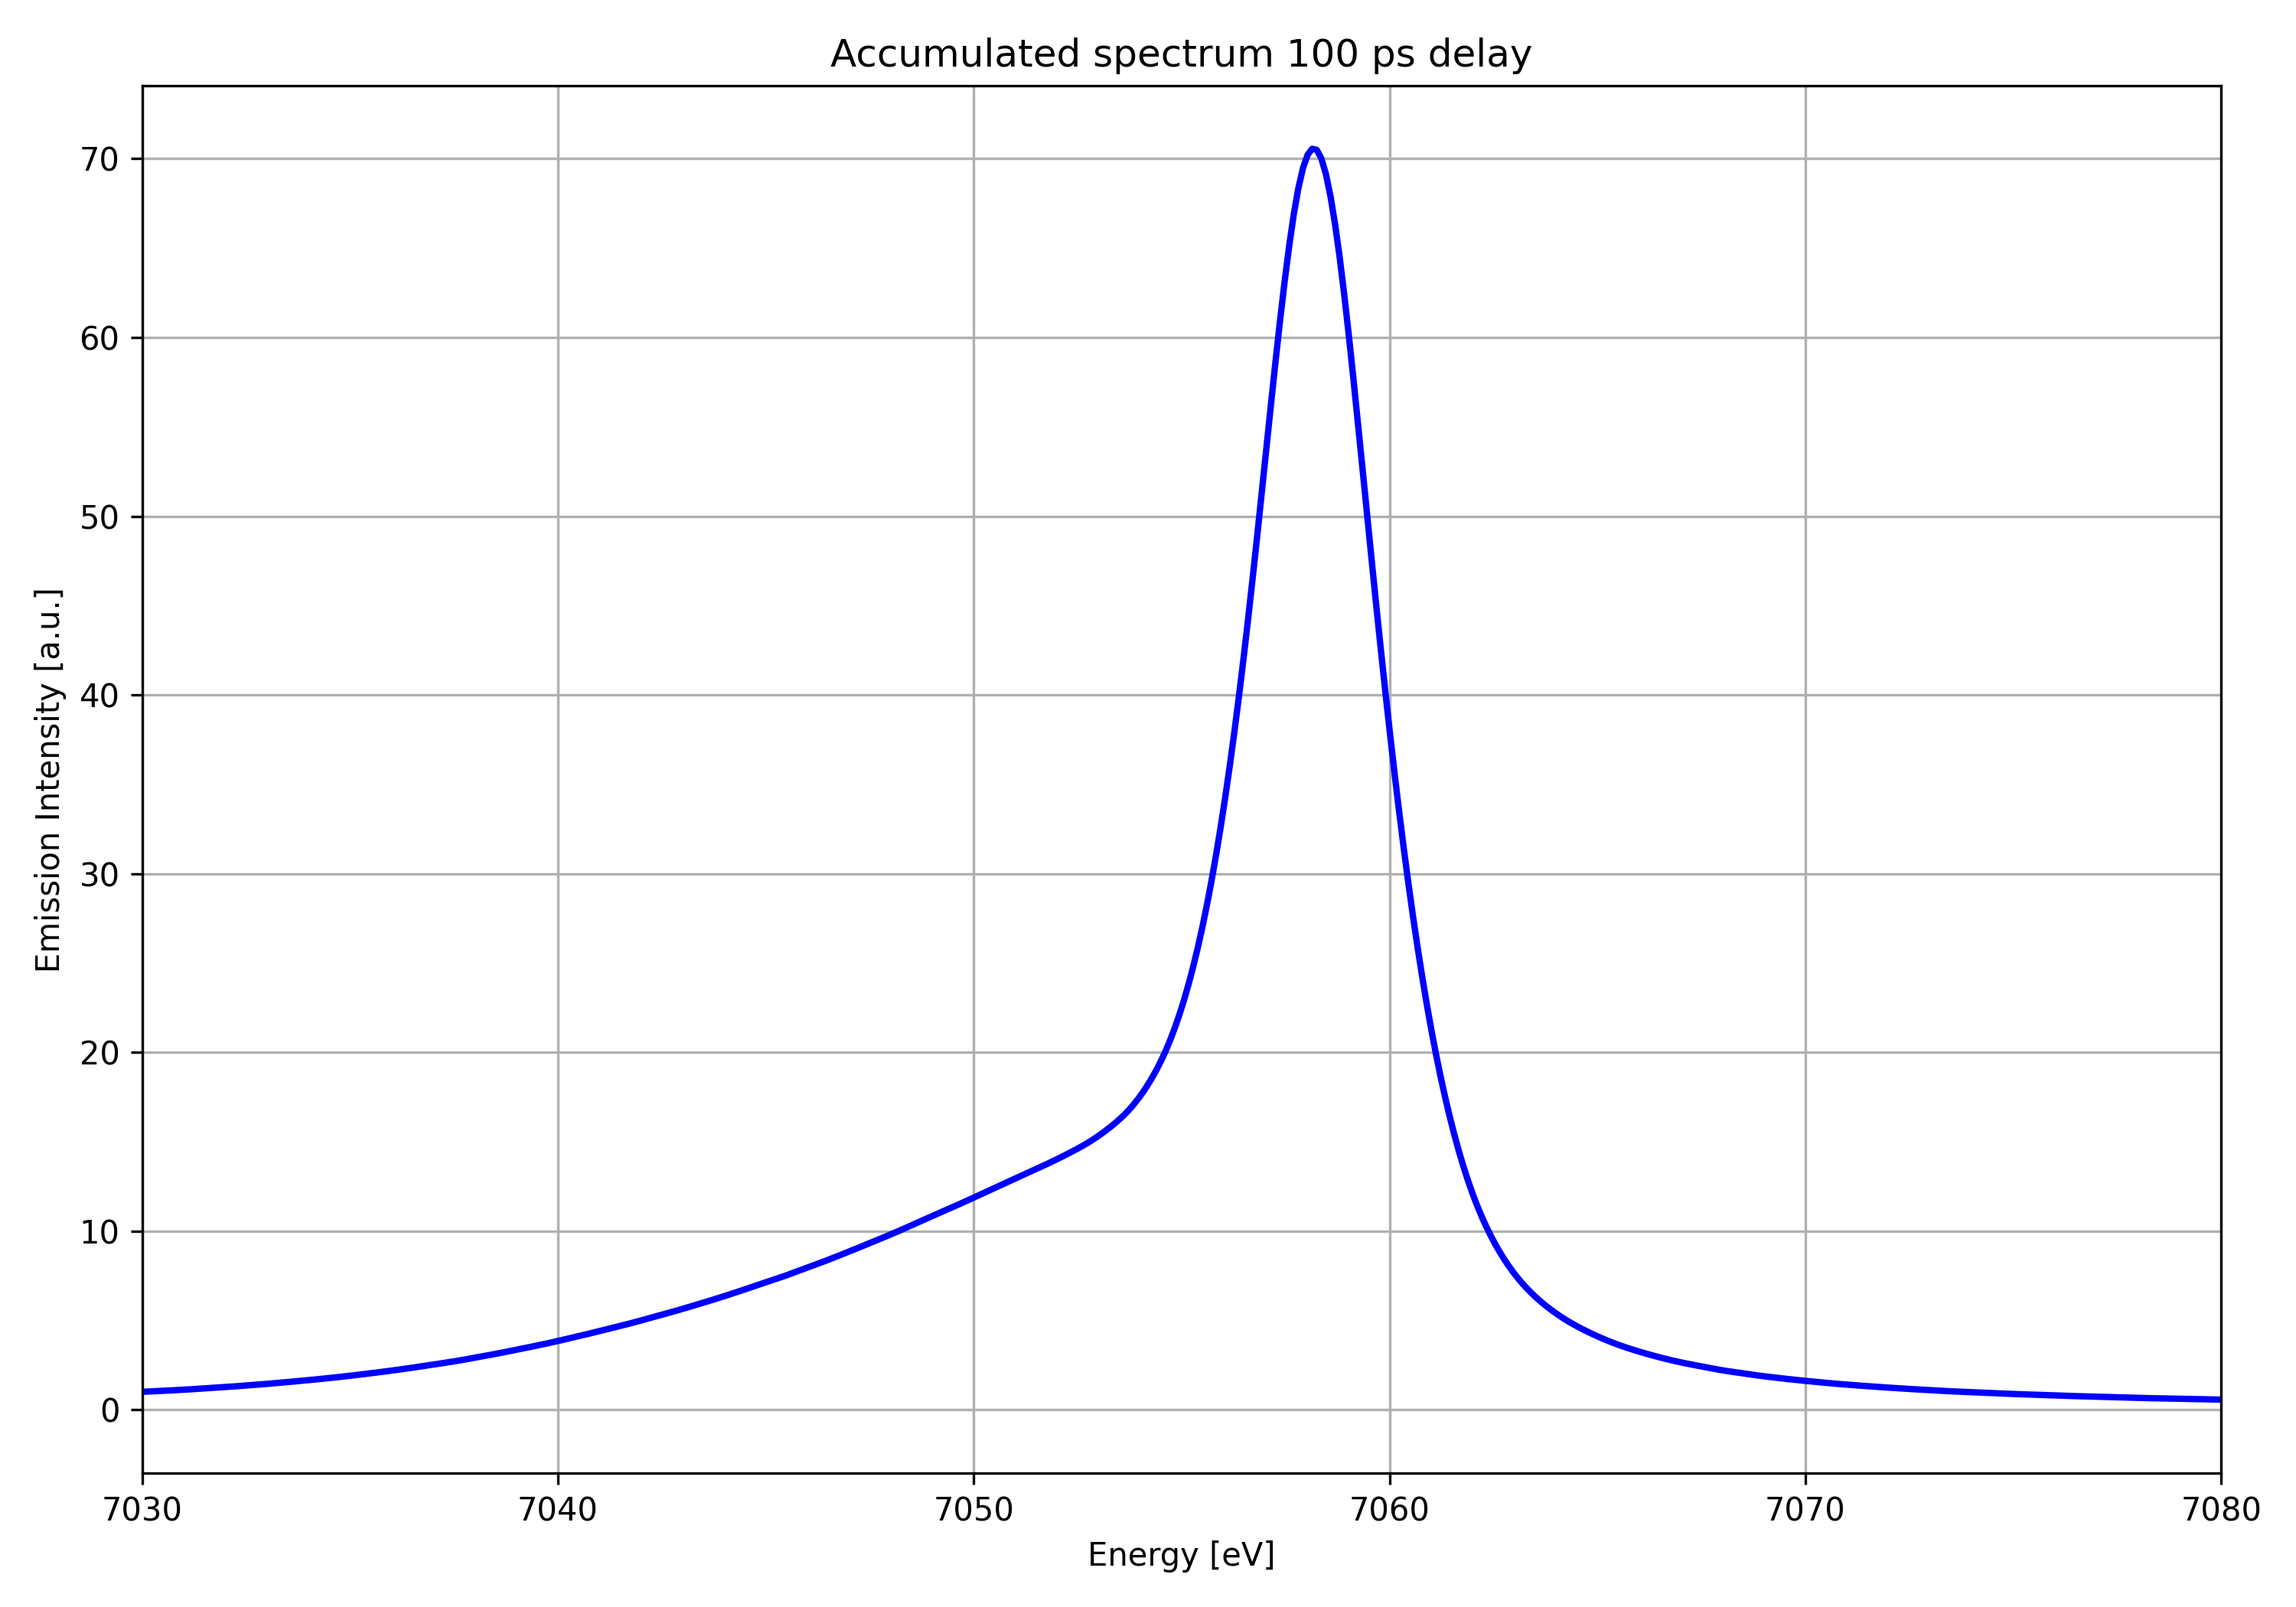
\includegraphics[width=\linewidth]{img/spectra/100ps spektrum.png}
        %\caption{XES spectrum with the excitation laser on at a delay of \qty{100}{ps}.}
        \label{fig:100ps spec}
    \end{subfigure}
    \hfill
    \begin{subfigure}[b]{0.45\textwidth}
        \centering
        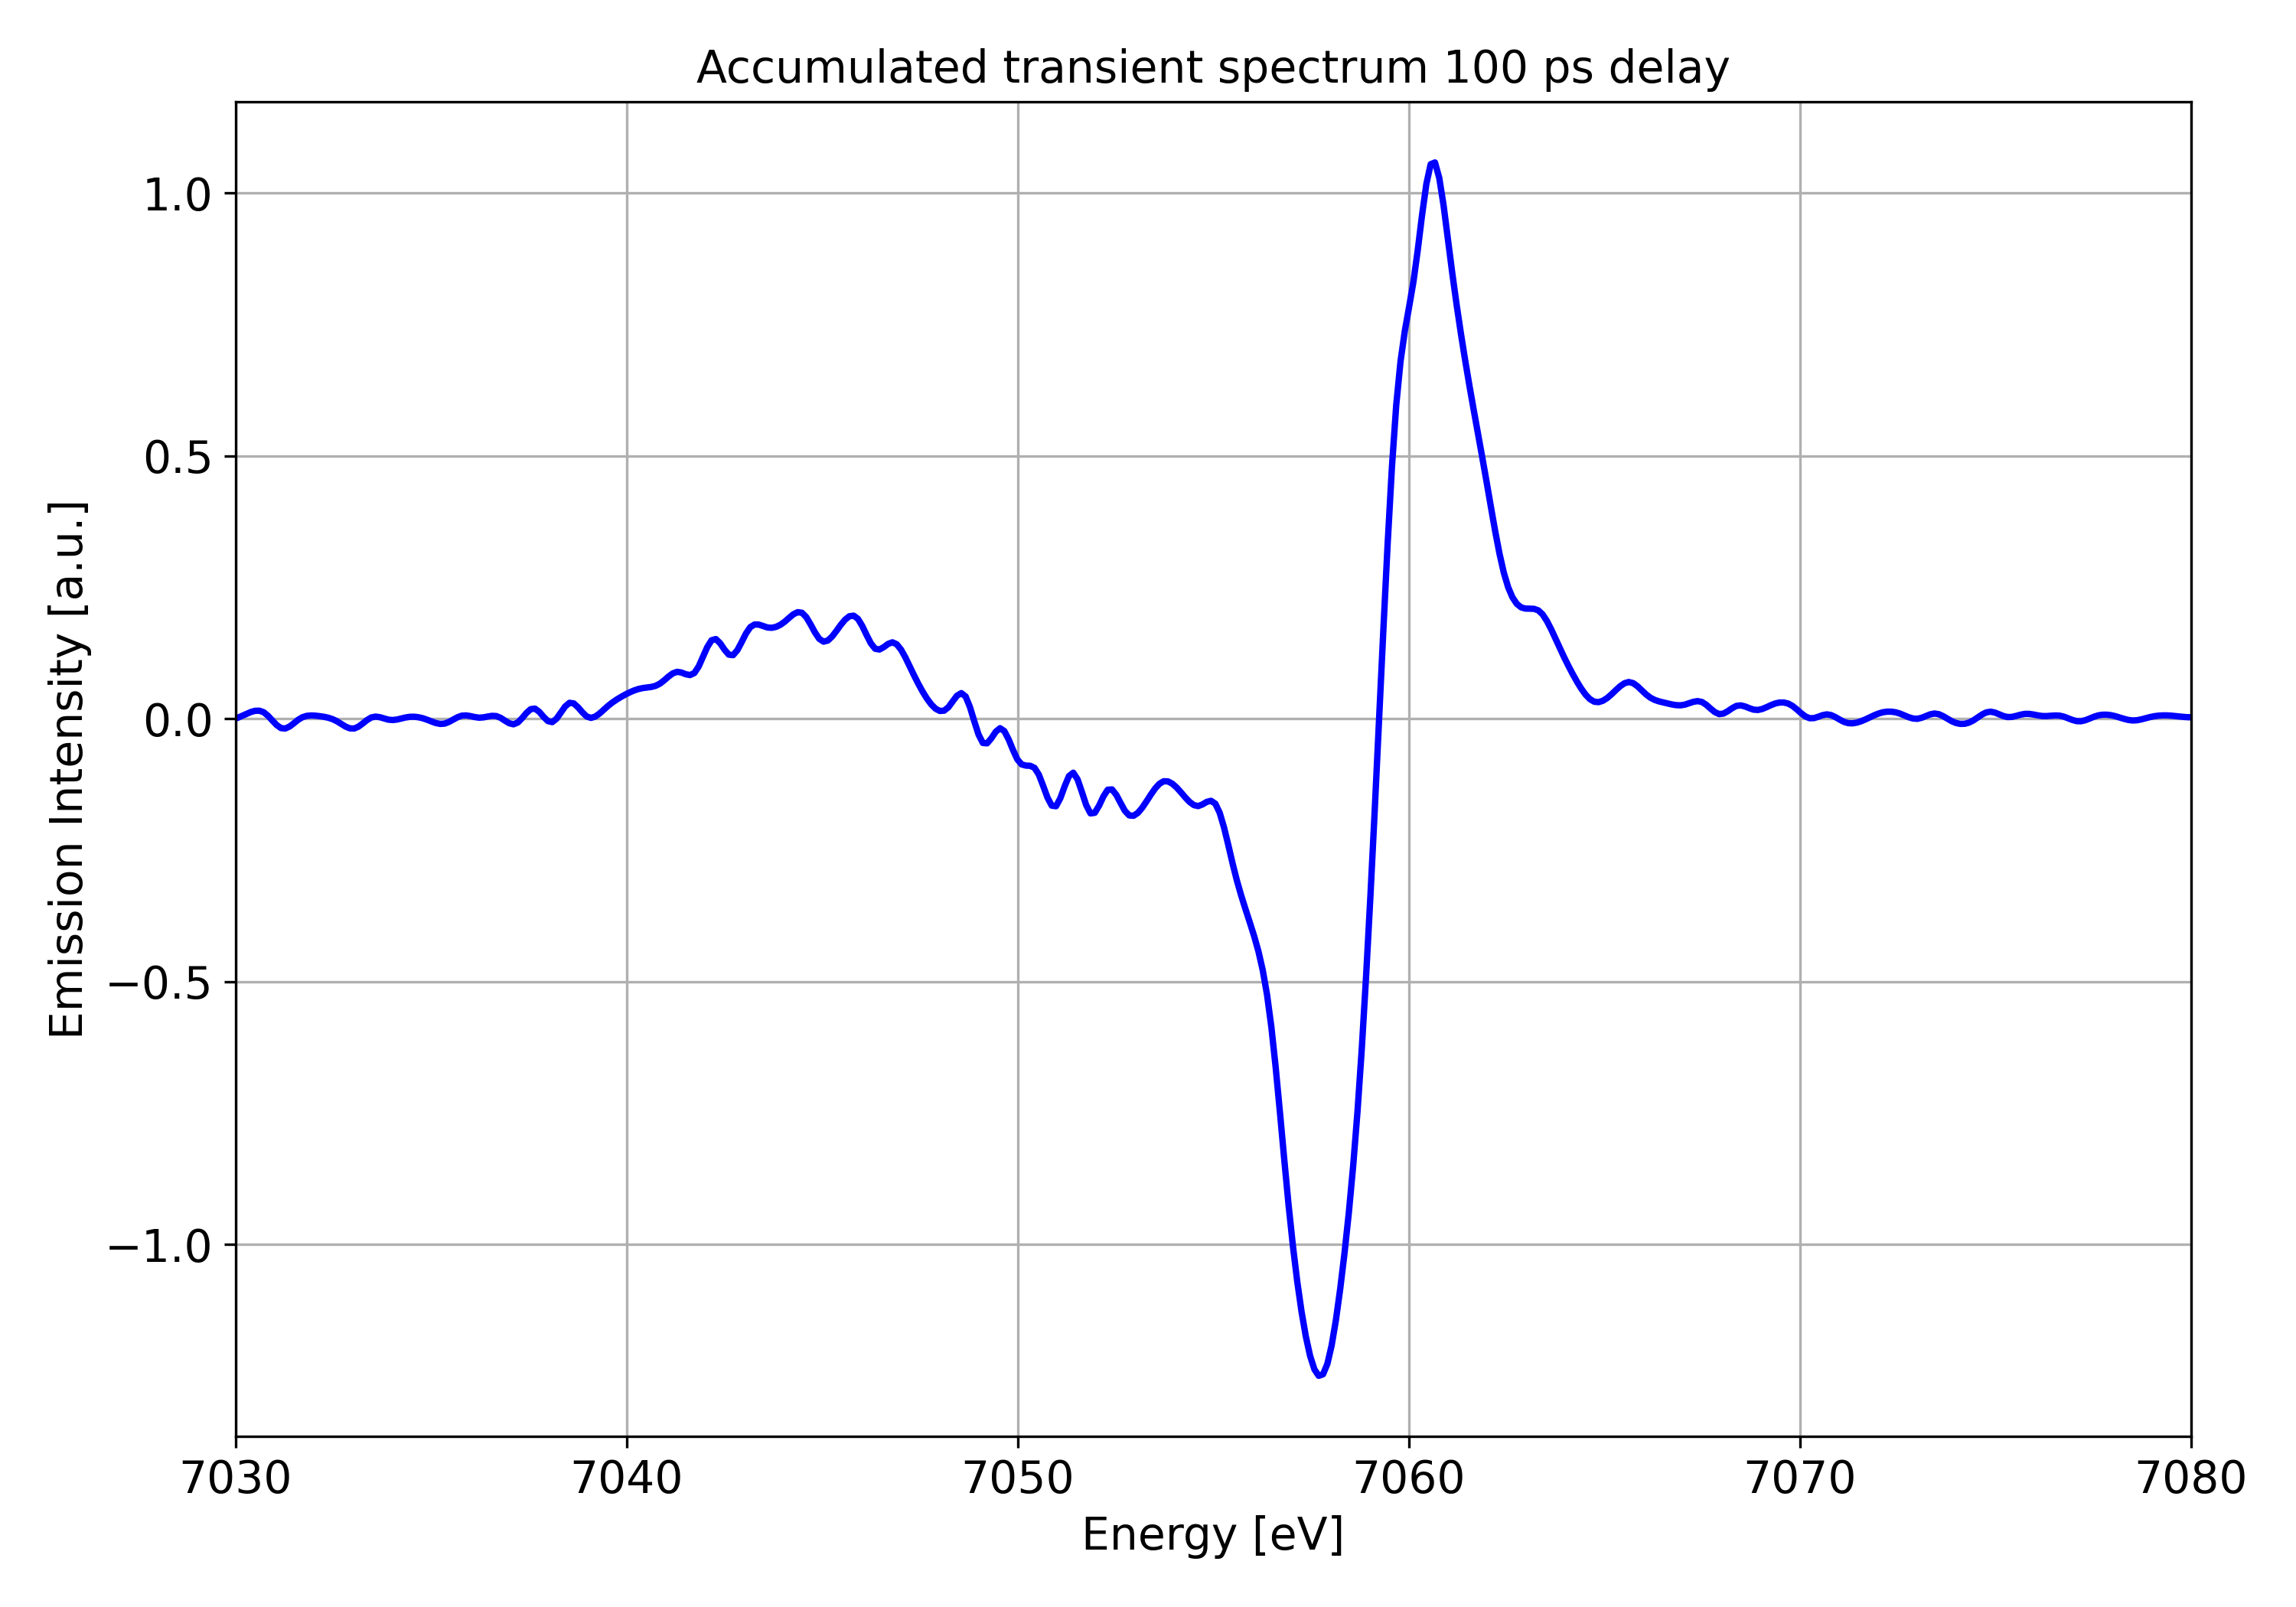
\includegraphics[width=\linewidth]{img/spectra/100ps diff spektrum.png}
        %diese grafiken müssen adjusted werden was größe der beschriftung angeht
        %\caption{Difference spectrum between a laser-off and laser-on measurement at a delay of \qty{100}{ps}.}
        \label{fig:100ps diff spec}
    \end{subfigure}
    \caption{On the left the XES spectrum with the excitation laser on at a delay of \qty{100}{ps} is plotted. On the right there's the difference spectrum at the same time delay.}
    \label{fig:100ps all spec}
\end{figure}

\subsection{Difference spectra for different pump-probe delays}
\begin{figure}[h]
     \centering
     
\includegraphics[scale=0.5]{img/Time_resolved_spectrum_errbars.png}
     \caption{Transient spectra of the X-ray emission at different pump-probe time delays.}
     \label{fig:time res spec}
\end{figure}
From the time resolved difference spectra of the measurements (see \autoref{fig:time res spec}) we can see multiple developments in the transient signal over the different time delays: at an energy around \qty{7045.0}{eV} the difference emission intensity grows (the intensity for the excited state is more intense than that of the ground state), at about \qty{7053.7}{eV} a shoulder in intensity difference initially emerges and then flattens out again for time delays $\Delta t>\qty{350}{fs}$. The two most prominent features of the transient signal are the minimum at \qty{7057.8}{eV} and the maximum at \qty{7060.5}{eV} which both match up with the difference spectrum provided.\\
Another thing to note is how little the change in spectrum between \qty{600}{fs} and \qty{800}{fs} is. The reaction has clearly landed on a more stable state, even though we can tell that it is still an excited state when comparing to the reference spectrum as it most closely matches the quintet-singlet transition denoted there. The comparison with the reference specrtum also tells us that there likely is a short-lived intermediate state as the shoulder we see resembles the triplet or quartet spectra.\\\\
\begin{figure}[h]
     \centering
     
\includegraphics[scale=0.5]{img/Kinetic traces.png}
     \caption{Kinetic traces at selected emission energies.}
     \label{fig:kin traces}
\end{figure}
The kinetic traces at these energies (see \autoref{fig:kin traces}) can be used to determine the rise time of the population of the excited states of $[\text{Fe}(\text{bipy})_3]^{2+}$ during the relaxation. To do this we use a function to parametise our reference spectrum:
\begin{align}
	S(E)=A\cdot\sum^5_{s=1}f_s\cdot S_s(E)
\end{align}
With $A$ being the amplitude, $s=\{1,2,3,4,5\}$ describing the multiplicity and $f_s$ being the population coefficients of the corresponding reference spectra $S_s(E)$. This means the population of the ground state - the singlet state - is described through $f_1$.\\
The population $T$ of our difference spectrum can now be described as:
\begin{align}
	T(E)=S(E)-S_1(E)=A\cdot\left(\sum^5_{s=1} f_s \cdot S_s(E)-S_1(E)\right)
\end{align}
The fitting function can be found in \autoref{py:fit}.\\
\begin{figure}[h]
     \centering
     
\includegraphics[scale=0.5]{img/fit/fit_all.png}
     \caption{The population curves of the different spin states plotted against the time delay of the optical laser in femtoseconds.}
     \label{fig:pop bigerr}
\end{figure}
Now that we have a fit for the time-dependant population of the respective states present during the different time delays (see \autoref{fig:pop bigerr}), we can see that our population curves have huge errorbars for the time delays $\Delta t\leq0$. This explains the occurence of any spin multiplicity other than singlet for our negative delays, as they should not occur. Our data is noisy for these delays and the fitting function struggles to get a read on the data.\\
To confirm this, we looked at the squared errors over the negative time delays (see \autoref{fig:counts}) and surmised that our photon count was much too low to justify the peaks seen in our popukation curve. This is also corroborated by looking at the residuals together with the measurements and seeing how noisy the measurements for a time delay of $\Delta t\leq0$ are in comparison to the one at \qty{50}{fs} (see \autoref{fig:resids}).
\begin{figure}[h]
     \centering
     
\includegraphics[scale=0.5]{img/fit/residuals_and_spectra_minus150_to_50fs.png}
     \caption{The normalised residuals together with the actual measurements and a fit over ... for time delays of $\Delta t=\{\qty{-150}{fs},\qty{-100}{fs},\qty{-50}{fs},\qty{0}{fs},\qty{50}{fs}\}$}
     \label{fig:resids}
\end{figure}
We then used this information to fix our population curves (see \autoref{fig:pop fixed}) by ...%ich check den code v6 noch nicht ganz
\begin{figure}[h]
     \centering
     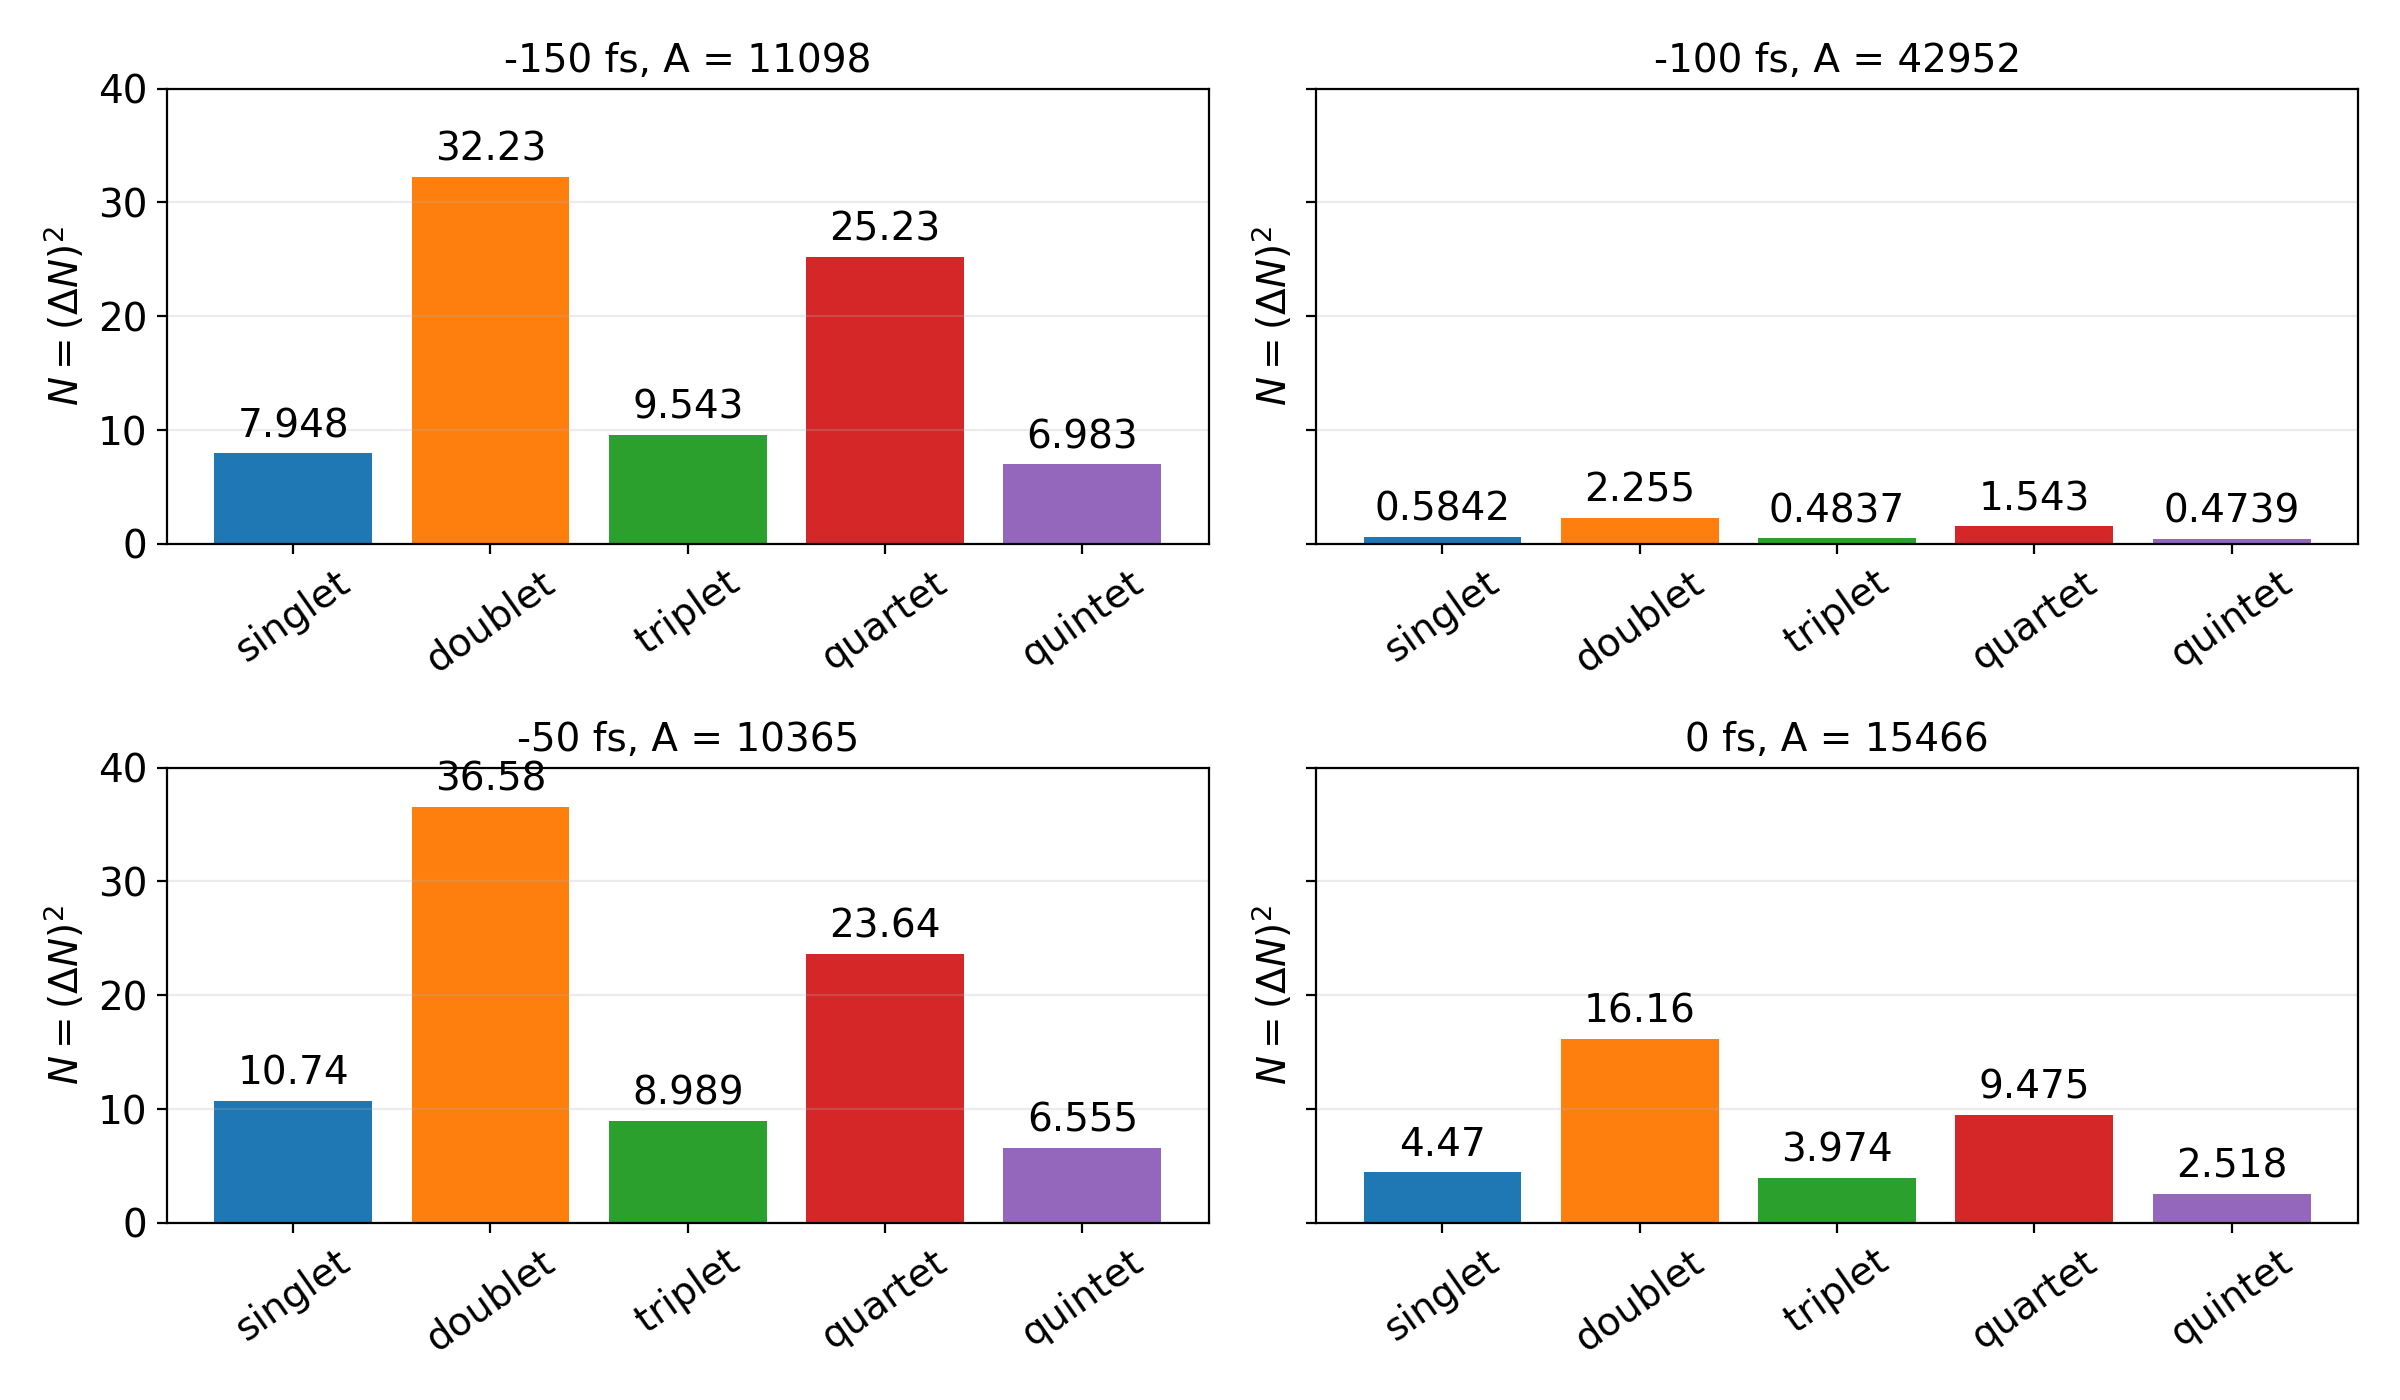
\includegraphics[scale=0.5]{img/fit/counts_negative_delays_per_delay.png}
     \caption{The photon counts of the different excited states for negative time delays.}
     \label{fig:counts}
\end{figure}

\begin{figure}[h]
     \centering
     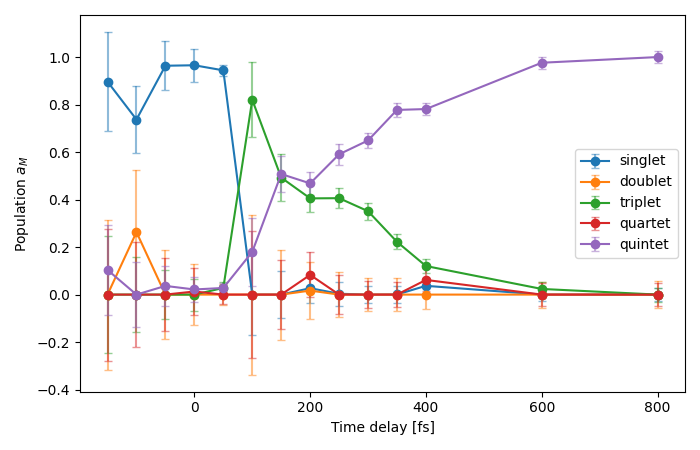
\includegraphics[scale=0.5]{img/fit/fit_try_to_fix_lol.png}
     \caption{The adjusted population curves of the different spin states plotted against the time delay of the optical laser in femtoseconds.}
     \label{fig:pop fixed}
\end{figure}
With this version of our fit we can see that nothing really changed for our positive delays. We see a population change from majority singlet to almost no singlets around our \qty{50}{fs} and \qty{100}{fs} delay with only small peaks at later delays with errorbars too big to really be definite peaks. Our triplet population grows rapidly for our \qty{100}{fs} delay which is a bit late when compared to our literature value $\tau<\qty{100}{fs}$ for our lifetime of the MLCT state, but still roughly in the order of magnitude. After that peak our triplet population steadily decreases and is overtaken by the quintet population which grows steadily from a delay of \qty{50}{fs}. At our latest time delay of \qty{800}{fs} the population is made up of almost only quintets with all other states being near 0. The doublet and quartet populations are near 0 for almost all time delays which is to be expected with the predicted intermediate states of the reaction. That they still exist is a result of ...%forgot :/



\section{Discussion of the physical meaning}


\section{Conclusion and Outlook}


\newpage

\pagenumbering{Alph}

\bibliographystyle{ieeetr}
\bibliography{literatur}

\newpage

\listoffigures 
\addcontentsline{toc}{section}{Abbildungsverzeichnis}

\newpage

\begin{appendices}
    
\section{Tabellen}

\section{VLab}
\label{Anh: VLab}

\section{Code}
%\lstinputlisting[language=Python]{Auswertung exp21.py}


\end{appendices}


\end{document} 